\chapter{\label{intro}Introduction}


In recent years, the control system has assumed an increasingly important role in developing and advancing modern civilization and technology. Practically every aspect of our day-to-day activities is affected by some control systems. Automatic control systems are abundant in all industry sectors, such as quality control of manufactured products, automated assembly lines, machine-tool control, space technology, weapon systems, computer control, transportation systems, power systems, robotics, etc. It is essential in such industrial operations as controlling pressure, temperature, humidity, and flow in the process 
industries. 
 
Recent application of modern control theory includes such non-engineering systems 
as biological, biomedical, control of inventory, economic and socio-economic systems. 
 
The basic ingredients of a control system can be described by:
\begin{itemize}
	\item Objectives of control. 
	\item Control system components. 
	\item Results or output. 
\end{itemize} 


\section{Automatic Controllers}

An automatic controller is used to compare the actual value of plant result with reference command, determines the difference, and produces a control signal that will reduce this difference to a negligible value. How the automatic controller has such a control signal is called the control action. 
 
An industrial control system comprises an automatic controller, an actuator, a plant, and a sensor (measuring element). The controller detects the actuating error command, usually at a shallow power level, and amplifies it to a very high level. The output of the automatic controller is fed to an actuator, such as a hydraulic motor, an electric motor, or a pneumatic motor or valve (or any other sources of energy). The actuator is a power device that produces input to the plant according to the control signal so that the output signal will point to the reference input signal. 
 
The sensor or the measuring element is a device that converts the output variable into another optimum variable, such as a displacement, pressure, or voltage, that can compare the output to the reference input command. This element is in a feedback path of the closed-loop system. The setpoint controller must be converted to reference input with the same unit as 
the feedback signal from the sensor element.

\section{Classification of Industrial controllers}
 
 Industrial controllers may be classified according to their control action as: 
\begin{itemize}
\item Two-position or on-off controllers 
\item Proportional controllers 
\item Integral controllers 
\item Proportional-plus-integral controllers 
\item Proportional-plus-derivative controllers 
\item Proportional-plus-integral-plus-derivative controllers 
\end{itemize}
 
The type of controller to use must be decided depending upon the nature of the plant and 
the operating condition, including such consideration as safety, cost, availability, 
reliability, accuracy, weight, and size. 
 
Two-position or on-off controllers:- 
 
In a two-position control system, the actuating part has only two fixed positions, which are, in many simple cases, simply on and off. Due to its simplicity and inexpensiveness, it is very widely used in both industrial and domestic 
control system.

Let the output signal from the controller be $\mathrm{u}(\mathrm{t})$ and the actuating error signal be $\mathrm{e}(\mathrm{t})$. Then mathematically,
$$
\begin{aligned}
&\mathrm{u}(\mathrm{t})=\mathrm{U}_{1}, \text { for } \mathrm{e}(\mathrm{t})>0 \\
&=\mathrm{U}_{2}, \text { for } \mathrm{e}(\mathrm{t})<0
\end{aligned}
$$
Where $\mathrm{U}_{1}$ and $\mathrm{U}_{2}$ are constants, and the minimum value of $\mathrm{U}_{2}$ is usually either zero or - U1.

\section{Proportional Control}

A proportional control system is a type of linear feedback control system. 
Proportional control is how most drivers control the speed of a car. If the car is at 
target speed and the speed increases slightly, the power is reduced slightly, or in 
proportion to the error (the actual versus target speed), so that the car reduces speed 
gradually and reaches the target point with very little, if any, "overshoot," so the result 
is much smoother control than on-off control. 
In the proportional control algorithm, the controller output is proportional to the error signal, which is the difference between the setpoint and the process variable. In other words, the output of a proportional controller is the multiplication product of the error signal and the proportional gain. This can be mathematically expressed as 

$$
\mathrm{P}_{\text {out }}=\mathrm{K}_{\mathrm{p}} \mathrm{e}(\mathrm{t})
$$
Where \\
$P_{\text {out }}$ : Output of the proportional controller \\
$K_{p}$ : Proportional gain \\
$e(t)$: Instantaneous process error at time ' $\mathrm{t}^{\prime} . e(t)=S P-P V$ \\
$S P$ : Set point \\
$P V$ : Process variable \\
With increase in $\mathrm{K}_{\mathrm{p}}$ : 
\begin{itemize}
	\item Response speed of the system increases.
	\item Overshoot of the closed-loop system increases. 
	\item Steady-state error decreases.
\end{itemize}
But with a high $K_p$ value, the closed-loop system becomes unstable.


\section{Integral Control}
 
In a proportional control of a plant whose transfer function doesn't possess an integrator 1/s, there is a steady-state error or offset in response to a step input. 
Such an offset can be eliminated if the integral controller is included in the system. 
 
In the integral control of a plant, the control signal, the output signal from the 
controller, at any instant, is the area under the actuating error signal curve up to that 
instant. But while removing the steady-state error, it may lead to an oscillatory response 
of slowly decreasing amplitude or even increasing amplitude, both of which is usually 
undesirable [5].


\section{Proportional-plus-integral controllers}

In control engineering, a PI Controller (proportional-integral controller) is a feedback controller which drives the plant to be controlled by a weighted sum of the error (difference between the output and desired setpoint) and the integral of that value. It is a special case of the PID controller in which the derivative (D) part of the error is not used.
The PI controller is mathematically denoted as:
$$
\mathrm{G}_{\mathrm{c}}=\mathrm{K}_{\mathrm{p}}+\frac{\mathrm{Ki}}{\mathrm{s}}
$$
or
$$
\mathrm{G}_{\mathrm{c}}=\mathrm{K}_{\mathrm{p}}\left(1+\frac{1}{\mathrm{sT}_{\mathrm{i}}}\right)
$$

\begin{figure}[H]
	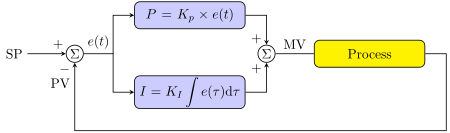
\includegraphics[width= \textwidth]{Basic block of PI Controller.svg.png}
	\caption{Basic block of PI Controller}
\end{figure}


Integral control action added to the proportional controller converts the original system into high order. Hence the control system may become unstable for a large value of $K_p$ since roots of the characteristic eqn. It may have a positive real part. In this control, proportional control action tends to stabilize the system, while the integral control action tends to eliminate or reduce steady-state error in response to various inputs. As the value of $T_i$ is increased, 
\begin{itemize}
\item Overshoot tends to be smaller 
\item Speed of the response tends to be slower. 
\end{itemize}


\section{Proportional-plus-derivative controllers}

Proportional-Derivative or PD control combines proportional control and derivative control in parallel. Derivative action acts on the derivative or rate of change of the control error. This provides a fast response, as opposed to the integral action, but cannot accommodate constant errors (i.e., the derivative of a constant, nonzero error is 0 ). Derivatives have a phase of $+90$ degrees leading to an anticipatory or predictive response. However, derivative control will produce large control signals in response to high-frequency control errors such as set point changes (step command) and measurement noise [5].

In order to use derivative control, the transfer functions must be proper. This often requires a pole to be added to the controller.
$$
\begin{aligned}
&\mathrm{G}_{\mathrm{pd}}(\mathrm{s})=\mathrm{K}_{\mathrm{p}}+\mathrm{K}_{\mathrm{d}} \mathrm{s} \text { or } \\
&=\mathrm{K}_{\mathrm{p}}\left(1+\mathrm{T}_{\mathrm{d}} \mathrm{s}\right)
\end{aligned}
$$
With the increase of $\mathrm{T}_{\mathrm{d}}$
\begin{itemize}
	\item Overshoot tends to be smaller
	\item Slower rise time but similar settling time.
\end{itemize}

\section{Proportional-plus-integral-plus-derivative controllers}

The PID controller was first placed on the market in 1939 and has remained the most widely used controller in process control until today. An investigation performed in 1989 in Japan indicated that more than 90\% of the controllers used in process industries are PID controllers and advanced versions of the PID controller. PI controllers are fairly common since derivative action is sensitive to measurement noise 

"PID control" is the feedback control method that uses the PID controller as the main tool. The basic structure of conventional feedback control systems is shown below, using a block diagram representation. In this figure, the process is the object to be controlled. The purpose of control is to make the process variable $y$ follow the setpoint value $r$. To achieve this purpose, the manipulated variable $u$ is changed at the command of the controller. As an example of processes, consider a heating tank where some liquid is heated to the desired temperature by burning fuel gas. The process variable $y$ is the temperature of the liquid, and the manipulated variable $u$ is the flow of the fuel gas. The "disturbance" is any factor other than the manipulated variable that influences the process variable. The figure below assumes that only one disturbance is added to the manipulated variable. However, in some applications, a major disturbance enters the process differently, or plural disturbances need to be considered. The error $e$ is defined by $e=r-y .$ The compensator $C(s)$ is the computational rule that determines the manipulated variable $u$ based on its input data, which is the error $e$ in the case of the figure. The last thing to notice about the figure is that the process variable $y$ is assumed to be measured by the detector, which is not shown explicitly here, with sufficient accuracy instantaneously that the input to the controller can be regarded as being exactly equal to $y$.

\begin{figure}[H]
	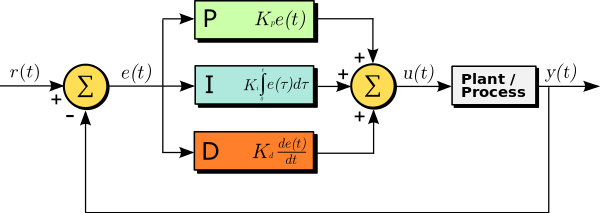
\includegraphics[width=\textwidth]{PID_en.svg.png}
	\caption{courtesy}
\end{figure}

When used in this manner, the three-element of PID produces outputs with the 
following nature:
\begin{itemize}
	\item $P$ element: proportional to the error at the instant t, this is the "present" error.
	\item $I$ element: proportional to the integral of the error up to the instant t, which can be interpreted as the accumulation of the "past" error. 
	\item $D$ element: proportional to the derivative of the error at the instant t, which can be interpreted as predicting the "future" error. 
\end{itemize}

Thus, the PID controller can be understood as a controller that considers the present, the past, and the future of the error. The transfer function $\mathrm{G}_{\mathrm{c}}(s)$ of the PID controller is :
$$
\begin{gathered}
\mathrm{G}_{\mathrm{c}}(\mathrm{s})=\mathrm{K}_{\mathrm{p}}\left(1+\frac{1}{\mathrm{ST}_{\mathrm{i}}}+\mathrm{T}_{\mathrm{d}} \mathrm{s}\right) \\
=\mathrm{K}_{\mathrm{p}}+\frac{\mathrm{K}_{\mathrm{i}}}{\mathrm{S}}+\mathrm{K}_{\mathrm{d}} \mathrm{s}
\end{gathered}
$$

\section{Application}	

In the early history of automatic process control, the PID controller was implemented as a mechanical device. These mechanical controllers used a lever, spring, and mass and were often energized by compressed air. These pneumatic controllers were once the industry standard .  Electronic analog controllers can be made from a solid-state or tube amplifier, a capacitor, and a resistance. Electronic analog PID control loops were often found within more complex electronic systems, for example, the head positioning of a disk drive, the power conditioning of a power supply, or even the movement-detection circuit of a modern seismometer. Nowadays, electronic controllers have largely been replaced by digital controllers implemented with microcontrollers or FPGAs.  Most modern PID controllers in the industry are implemented in programmable logic controllers (PLCs) or as a panel-mounted digital controller. Software implementations have the advantages that they are relatively cheap and are flexible with respect to the implementation of the PID algorithm [5]

\setcounter{equation}{0}
\setcounter{table}{0}
\setcounter{figure}{0}
%\baselineskip 24pt


 



